\section{Implementation}\label{sec:cicada_eval} 

\subsection{Parameter Settings}

In this section, we evaluate the practicality and optimality of various HTLP constructions based on the parameters $M,n,m,w$ of the auction or vote. 
% As discussed in~\Cref{sec:packing}, the size of the applied integer representations of ballots/bids increases linearly in certain parameters of the voting/auction schemes, e.g., the number of candidates. This limits the applicability of certain HTLP constructions instantiated in specific cryptographic groups, as we show next.  
Assuming the classic PNS packing, we require $(nw+1)^m\leq\vert\mathbb{G}\vert$ for voting and $M^n\leq\vert\mathbb{G}\vert$ for auctions, where $\mathbb{G}$ is the group in which the HTLP is instantiated.
We show the optimal HTLP construction for auctions and voting for various parameter settings in \Cref{fig:packed_feasibility} (with packing) and \Cref{fig:nopack_feasibility} (without packing). We use the security parameter $\secpar=80$ (see discussion in \Cref{sec:implementation}), which corresponds to a $1024$-bit modulus $N$ for exponential ElGamal and Paillier HTLPs and $3400$-bit discriminants for class group HTLPs. For the exponential ElGamal HTLP, we fixed the maximum ballot at $2^{80}$, which corresponds to $\approx 2^{40}$ brute-forcing work using Pollard's rho algorithm~\cite{Pollard78}.

\begin{figure}[tb!]
    \centering
    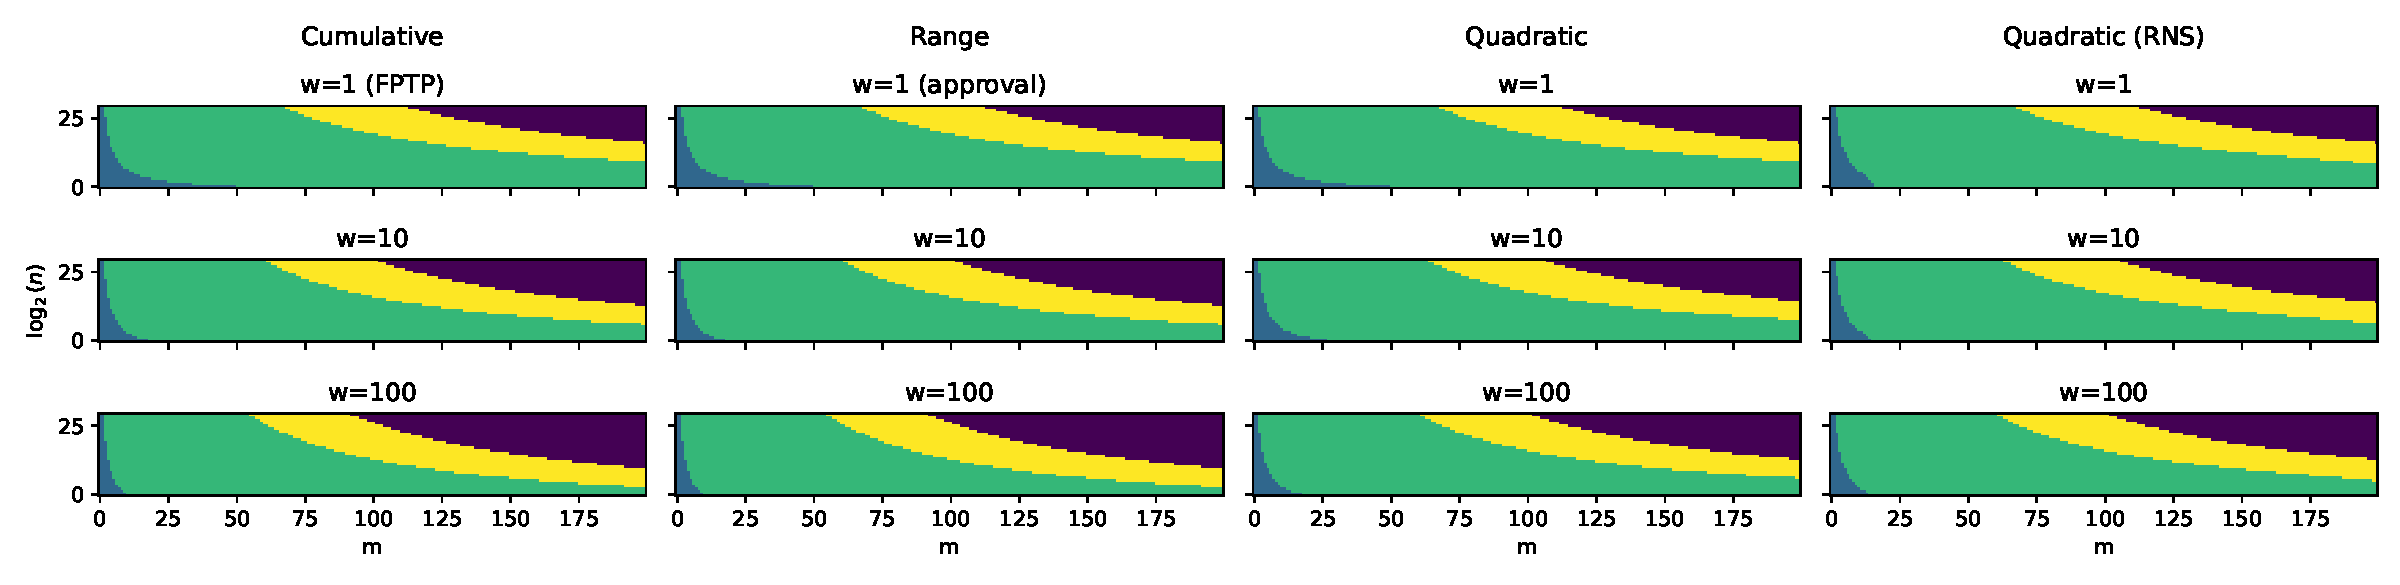
\includegraphics[width=\textwidth]{cicada/figs/params/pack_crq.pdf}
% \includegraphics[scale=0.56,trim={0.5cm 3cm 0.2cm 4.5cm},clip]
    \centering  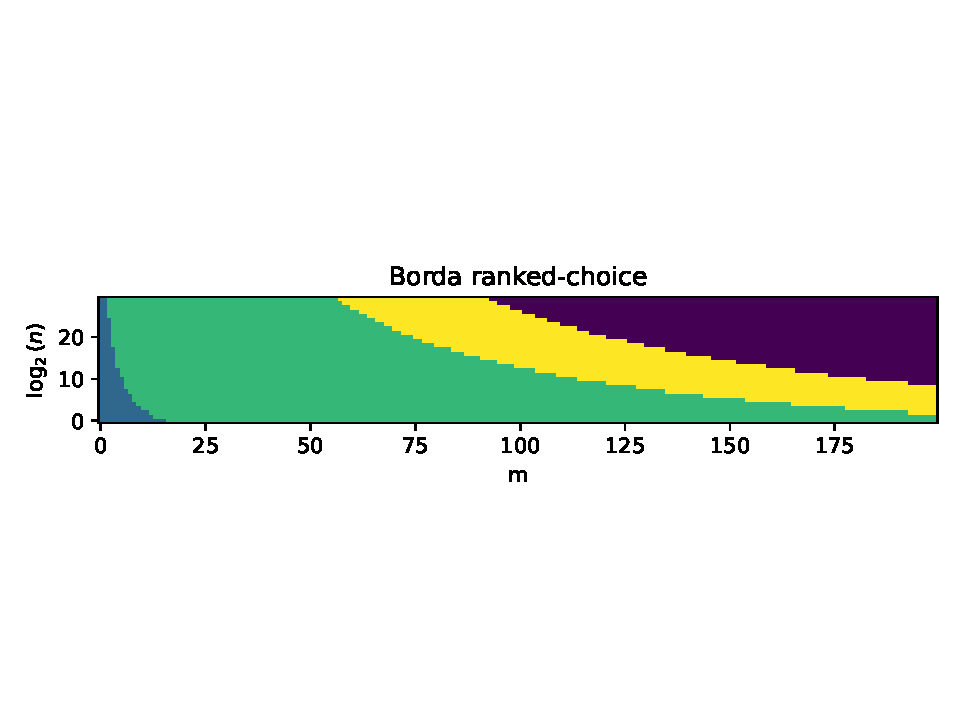
\includegraphics[width=0.45\textwidth,trim={0cm 3cm 0cm 4.5cm},clip]{cicada/figs/params/pack_borda.pdf}  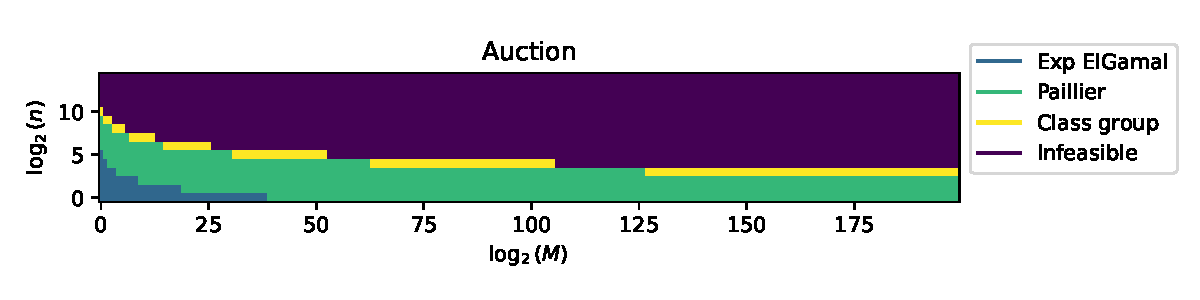
\includegraphics[width=0.5\textwidth,trim={0cm -1cm 0cm 4.5cm}]{cicada/figs/params/pack_auction.pdf}
    \caption{Most efficient HTLP construction for voting and auction using Cicada with maximal packing (using PNS except where indicated).}
    \label{fig:packed_feasibility}
\end{figure}

\begin{figure}[tb!]
    \centering
    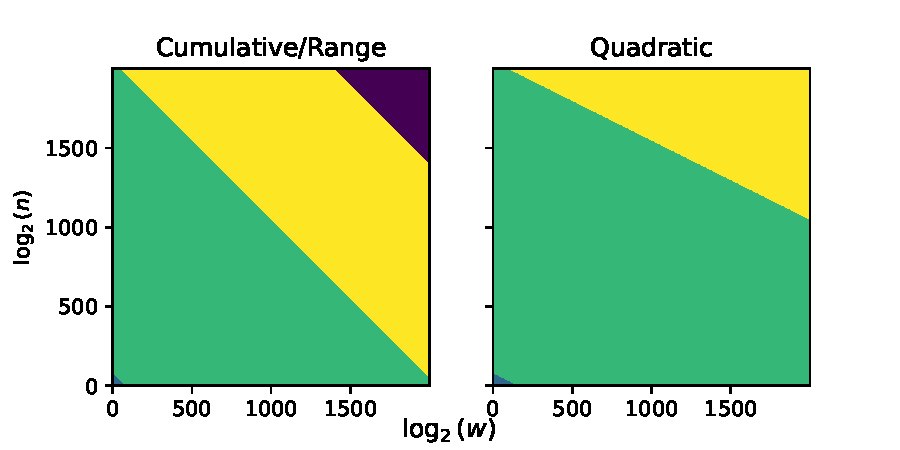
\includegraphics[width=0.49\textwidth,trim={0cm -0.5cm 0cm 0cm}]{cicada/figs/params/nopack_crq.pdf}
    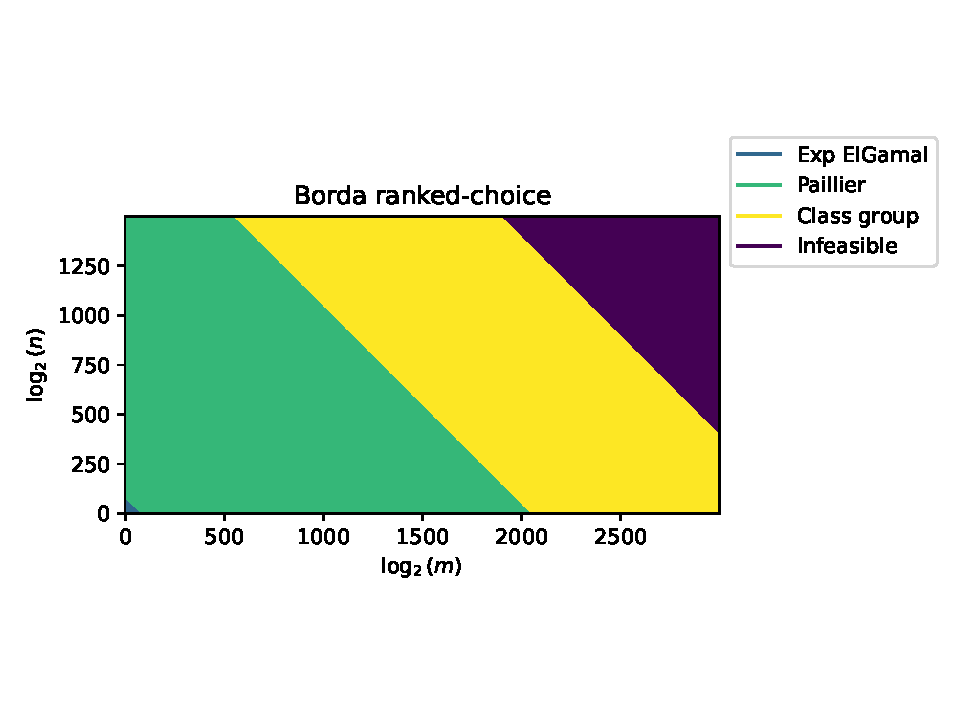
\includegraphics[width=0.49\textwidth,trim={2cm 2cm 0cm 2cm},clip]{cicada/figs/params/nopack_borda.pdf}
    \caption{Most efficient HTLP construction for voting schemes using Cicada without packing. For the sealed-bid auction, the bid bit-length directly determines the HTLP construction to use (exponential ElGamal up to 80 bits, then Paillier up to 2048, and class group up to 3400).}
    \label{fig:nopack_feasibility}
\end{figure}

\paragraph{Exponential ElGamal HTLP (\Cref{con:exp_elgamalHTLP})} 
This is the most efficient HTLP construction: for a given security parameter, it has the smallest required cryptographic groups and most efficient group operations. However, since the puzzle solution is encoded in the exponent, solving the puzzle requires brute-forcing a discrete logarithm. This limits the use of this construction to a small set of parameter settings: assuming the largest discrete logarithm an off-chain solver can be expected to brute-force has $\tau$ bits, we require $(nw+1)^m \leq 2^{2\tau}$.

\paragraph{Paillier HTLP (\Cref{con:paillierHTLP})} 
This is a slightly less efficient construction since the size of the HTLPs for a given security parameter is doubled due to working over $\bmod~N^2$ instead of $\bmod~N$. This increases both the required storage and the complexity of the group operation. On the other hand, due to its larger solution space, the Paillier HTLP supports much broader parameter settings for a given security parameter.

\paragraph{Class group HTLP} 
Class group offer the sole HTLP construction without a trusted setup~\cite{CCS:TCLM21}. This comes at the cost of the largest groups for a given security parameter. Class groups are not widely supported by major cryptographic libraries, and their costly group operation makes blockchain deployment difficult. We are unaware of any class group implementations for Ethereum smart contracts.

\paragraph{Impractical parameter settings} 
Accommodating very large settings of $n,\allowbreak w,m,M$ requires larger groups, leading to group operations and storage requirements which are intolerably inefficient for certain applications.

\subsection{Our Implementation}\label{sec:implementation}

We implemented our transparent on-chain coordinator as an Ethereum smart contract in Solidity.\footnote{Open-sourced at \url{https://github.com/a16z/cicada}.} 
For efficiency, we use the exponential ElGamal HTLP with a 1024-bit modulus $N$.
To enable 1024-bit modular arithmetic in $\ZZ_N^*$, we developed a Solidity library which may be of independent interest. 
This size of $N$ corresponds to approximately $\secpar=80$ bits of security.
Although this security level is no longer deemed cryptographically safe, the secrecy of the HTLP solutions is only guaranteed up to time $T$ regardless, so this security level will suffice for our use case as long as the best-known factoring attack takes at least $T$ time. A 2012 estimate for factoring 1024-bit integers is about a year~\cite{facthacks}, which is significantly longer than the typical submission period of a decentralized auction or election.

The main factors influencing gas cost (see \Cref{sec:cicada_costs}) are submission size, correctness proof size, and verification complexity. These factors mainly depend on the packing parameter $\ell\in[m]$, which determines a storage-computation trade-off with the following extremes:
% For the implementation, our main concern is minimizing the size of the ballots/bids, their correctness proofs, and the verification complexity of the correctness proofs. These metrics influence the gas cost efficiency of our transparent tallying authorities/auctioneers implemented as Ethereum smart contracts in Solidity. Our code is open-sourced.~\footnote{\url{https://github.com/a16z/cicada}\todo{anonymize}}

\begin{description}
    \item[One aggregate HTLP for all.] If $\ell=m$, the contract maintains a single aggregate HTLP $Z$. This greatly reduces the on-chain space requirements of the resulting voting or auction scheme at the expense of typically more complex and larger submission correctness proofs.
    \item[One aggregate HTLP per candidate.] If $\ell=1$, the contract must maintain $m$ aggregate HTLPs $\{Z_j\}_{j\in[m]}$. This increases the on-chain storage, but the submissions of correctness proofs become smaller and cheaper to verify.
\end{description}
In~\Cref{sec:cicada_costs}, we empirically explore this trade-off space by measuring the gas costs of various deployments of our framework with a range of parameter settings $M,n,m,w,\ell$.
% \joe{what about other points in the trade-off space?}
%\noemi{we don't actually measure any ``in-between'' settings of $\ell$ though, can we simulate or at least discuss whether it's linear?}\istvan{should be linear} 

First, we briefly describe the proof systems used for each scheme we implement; detailed descriptions are given in \Cref{sec:sigmas}.

\paragraph{Binary voting.} 
In a binary vote (i.e., approval voting with $m=1$), such as a simple yes/no referendum, users prove that the submitted ballot $Z=(u,v)$ is an exponential ElGamal HTLP with solution $0$ or $1$: $(u=g^r\land v=h^r)\lor(u=g^r\land vy^{-1}=h^r)$. This is achieved via OR-composition~\cite{C:CraDamSch94} of two sigma protocols for discrete logarithm equality~\cite{C:ChaPed92}.

\paragraph{Cumulative voting.}
In cumulative voting, each user distributes $w$ votes among $m$ candidates. To accommodate a larger number of candidates, our implementation keeps $m$ tally HTLPs $Z_j$, one for each candidate (in other words, $\ell = 1$). Each voter $i$ submits $m$ ballots $Z_{ij} = (g^{r_{ij}},h^{r_{ij}}y^{s_{ij}})$ for all $j\in[m]$. Besides proving (using the protocol \zkpoks) that each HTLP is well-formed (the same $r_{ij}$ is used in both terms), the voter must prove that $0 \leq s_{ij}~\forall\ j\in[m]$ and $\sum^m_{j=1} s_{ij}=w$. The first condition is shown with a proof of positive solution (\zkpopos) via Legendre's three-square decomposition theorem~\cite{ACNS:Groth05}. As a building block, we use a proof of square solution (\zkposqs) to show that a puzzle solution is a square. The second condition is proven by providing the randomness $R_i = \prod_j r_{ij}$ which opens $\prod_{j} Z_{ij}$ to $w$.

\paragraph{Sealed-bid auction.}
To illustrate two extremes of the packing spectrum, we implement two flavors of sealed-bid auctions. The first uses a single aggregate HTLP as described in \Cref{sec:cicada_framework} (this can be viewed as $\ell = b$, where $b = \ceil{\log_2(M)}$ is the bit-length of a bid): Bidder $i$ submits a single HTLP $Z_i = (g^{r_i},h^{r_i} y^{s_i})$, proving well-formedness with \zkpoks and two \zkpopos to show $0\leq s\leq M$. The coordinator aggregates the $i$th bidder's bid by adding $M^{i-1} \cdot Z_i$ to its tally.
% The coordinator will aggregate the $i$th bidder's bid by multiplying it by $2^{ib}$, where $b = \ceil{\log_2(M)}$ is the bit-length of the max bid $M$. That is each $b$-bit segment of the aggregate HTLP stores one bid. 

The second approach applies $b$ aggregate HTLPs (i.e., $\ell = 1$): Each bidder $i$ submits $b$ HTLPs $\{Z_{ij}\}_{j \in [b]}$ and uses the same proof system as in binary voting to prove their well-formedness, i.e., the user inserted for each bit of the bid $0$ or $1$. The coordinator adds $2^i \cdot Z_{ij}$ to each corresponding aggregate HTLP $Z_j$.%\footnote{We implement\noemi{check this} an optimization in which the bidders perform the scalar multiplication on behalf of the coordinator, proving instead $\forall j\in[b]$, $(u=g^r\land v=h^r)\lor(u=g^r\land vy^{-2^i}=h^r)$.\noemi{not sure if it's easy to discuss at which $M > 2$ this stops being more efficient than having the contract do the multiplication?}\istvan{doesn't the contract need to do the multiplication anyways because of security reasons? You cannot trust the user computing $y^{-2^i}$.}}\istvan{see signal conversation for more discussion on this.}
% We also describe the proof systems used for the implemented schemes in the full version.

\subsection{Deployment Costs}\label{sec:cicada_costs}

\begin{table*}[tb!]
    \makebox[\linewidth]{
    \centering
    \setlength{\tabcolsep}{6pt}
    \setlength{\belowbottomsep}{6pt}
    \begin{tabular}{l c ccccc}
        \toprule
        & \textbf{Binary vote} & \multicolumn{5}{c}{\textbf{Cumulative vote} ($\ell=1$)} \\\midrule
        $m$             & $1$ & $2$ & $3$ & $4$ & $5$ & $6$ \\\midrule
        \Aggr      & $418,358$ & $3,391,514$ & $5,081,542$ & $6,781,389$ & $8,489,786$ & $10,208,185$ \\
        \Finalize  & $115,690$ & $269,505$ &$397,789$&$521,895$&$644,814$&$770,934$ \\
        \midrule %%%%%%%%%%%%%%%%%%%%%%%%%%%%%%%%
        & \textbf{Sealed-bid auction} ($\ell = b$) & \multicolumn{5}{c}{\textbf{Sealed-bid auction} ($\ell=1$)} \\\midrule
        $b$                  & any & $8$ & $10$ & $12$ & $14$ & $16$ \\\midrule
        \Aggr                & $3,055,107$ & $3,586,022$ & $4,488,050$ & $5,394,047$ & $6,304,164$ & $7,218,905$ \\
        \Finalize            & $147,634$ & $1,005,208$ & $1,253,119$ & $1,497,760$ & $1,749,489$ & $2,003,282$ \\
        \bottomrule
    \end{tabular}
    }
    \caption{Gas costs for Cicada cumulative voting and sealed-bid auctions with various numbers of candidates $m$, bid bit-lengths $b$ (max. bid $M = 2^{b-1}$), and packing parameters $\ell$.}
    \label{tab:gas_table}
\end{table*}

We report EVM gas costs of several instantiations of Cicada in \Cref{tab:gas_table}. 

\paragraph{Submission costs} 
The on-chain cost of submitting a bid/ballot is the cost of running the $\sf Aggr$ function by the contract, i.e., the verification of the well-formedness proofs plus adding the users' submissions to the tally HTLPs (if and only if they verify). We report our measurements without packing (i.e., $\ell=1$). Submitting a binary vote ballot costs $418,358$ gas ($\approx 15.36$ USD on Ethereum).\footnote{We can estimate gas costs for approval voting using the cost of binary voting, as the former uses a disjunction of $m$ copies of the same NIZK and thus scales linearly.} 
For cumulative voting, the submission cost scales linearly in $m$: with $m=2$ candidates, submitting a ballot costs 
$3,391,514$ gas ($\approx124.51$ USD), 
and each additional candidate adds $\approx 1,699,847$ gas ($\approx 62.40$ USD).

An auction with a single HTLP for each bit of the bid (the $\ell=1$ case) requires a submission cost of $3,586,022$ gas ($\approx94.49$ USD) for an $8$-bit bid. Every additional bit in the submitted bid burns $\approx451,014$ gas ($\approx 11.89$ USD). 
On the other hand, if one applies packing, i.e., $\ell=b$, then the cost of submitting a sealed bid is constant at $3,055,107$ gas ($\approx131.65$ USD). With bid-space $M=2^7$ it is already more economical to have a single aggregate HTLP and use a packing scheme, despite more complex bid-correctness proofs.

\paragraph{Finalization costs} 
Our voting and auction schemes end with solving the tally HTLP(s) off-chain, i.e., computing $(g^r)^{2^{\Ttime}}$. With exponential ElGamal, solving the puzzle also requires the off-chain solver to brute-force a discrete logarithm. The correctness of this computation is proven to the contract with Wesolowski's \poe~\cite{EC:Wesolowski19} (recalled in \Cref{sec:sigmas}). The $\Finalize$ cost comes from verifying the \poe(s) on-chain, which burns $101,066$ gas ($\approx3.71$ USD) per proof. Without packing, the untrusted solver must provide a Wesolowski proof per tally HTLP, so the $\Finalize$ gas cost is linear in the number of tally HTLPs. A portion of the Wesolowki verification cost comes from checking that the challenge is a prime number. Our implementation uses a Baillie-PSW~\cite{PomSelWag80} primality test, which costs $44,972$ gas ($\approx1.65$ USD). 

\begin{table}[ht]
    \centering
    \setlength{\tabcolsep}{6pt}
    % \setlength{\belowbottomsep}{6pt}
    \begin{tabular}{l r}
       \toprule
       \textbf{Sigma protocol}  & \textbf{Verification gas cost}\\
       \midrule
       Proof of Exponentiation (\poe~\cite{EC:Wesolowski19})& $101,066$\\
        PoK of solution (\zkpoks) & $266,096$ \\
        Proof of solution equality (\zkposeq) & $336,155$ \\
        Proof of square solution(\zkposqs) & $336,168$ \\
        Proof of positive solution (\zkpopos) & $1,351,958$ \\
        \bottomrule
    \end{tabular}
    \caption{EVM gas costs of verification for the proof systems described in~\Cref{sec:sigmas}.}
    \label{tab:sigmas_gas}
\end{table}

\paragraph{Verification costs}
Our Solidity implementation includes the sigma protocols described in \Cref{sec:sigmas}. We report their verification costs in~\Cref{tab:sigmas_gas}. With Groth's trick~\cite{ACNS:Groth05} in the proof of positivity (\zkpopos), we must decompose the integer solution into the sum of only three squares. Therefore, the gas cost of verifying \zkpopos equals the cost of verifying three proofs of knowledge of square solutions (\zkposqs) and one proof of knowledge of equal solution (\zkposeq).

\begin{table*}[ht!]
    % \adjustbox{width=1.2\textwidth,center}{
    \centering
    \setlength{\tabcolsep}{6pt}
    \setlength{\belowbottomsep}{6pt}
    \begin{tabular}{l SS}
        \toprule
        & {\textbf{Binary vote}} & {\textbf{Sealed-bid auction} ($\ell = b$)} \\\midrule
        & {$m=1$} & {$b=$ any} \\\midrule
        $\Aggr$\ (ETH L1)     & 15.36 & 112.16 \\
        $\Aggr$\ (Arbitrum Nova)      & 0.35 & 2.55 \\
        $\Aggr$\ (Optimism)      & 0.00918 & 0.06701 \\
        $\Aggr$\ (zkSync Era)     & 0.063 & 0.459 \\\midrule
        $\Finalize$\ (ETH L1)  & 4.25 & 5.42 \\
        $\Finalize$\ (Arbitrum Nova)  & 0.10 & 0.12 \\
        $\Finalize$\ (Optimism) & 0.00254 & 0.00324 \\
        $\Finalize$\ (zkSync Era)  & 0.017 & 0.022 \\
        \bottomrule
    \end{tabular}
    \caption{USD costs of Cicada binary vote and fully packed ($\ell=b$) sealed-bid auction on Ethereum L1, Arbitrum Nova, Optimism, and zkSync Era as of July 30, 2024 at 7:30 PM UTC.}
    \label{tab:usd_table1}
\end{table*}

\begin{table*}[ht!]
    % \makebox[\linewidth]{
    % \resizebox{1.2\textwidth}{!}{
    \adjustbox{width=1.2\textwidth,center}{
    \centering
    \setlength{\tabcolsep}{6pt}
    \setlength{\belowbottomsep}{6pt}
    \begin{tabular}{l SSSSS}
        \toprule
        & \multicolumn{5}{c}{\textbf{Cumulative vote} ($\ell=1$)} \\\midrule
        $m$             & {2} & {3} & {4} & {5} & {6} \\\midrule
        $\Aggr$\ (ETH L1)     & 124.51 & 186.55 & 248.95 & 311.67 & 374.75 \\
        $\Aggr$\ (Arbitrum Nova)      & 2.83 & 4.24 & 5.66 & 7.08 & 8.52 \\
        $\Aggr$\ (Optimism)      & 0.07439 & 0.11145 & 0.14874 & 0.18621 & 0.22390 \\
        $\Aggr$\ (zkSync Era)     & 0.509 & 0.763 & 1.018 & 1.275 & 1.533 \\\midrule
        $\Finalize$\ (ETH L1)  & 9.89 & 14.60 & 19.16 & 23.67 & 28.30 \\
        $\Finalize$\ (Arbitrum Nova)  & 0.22 & 0.33 & 0.44 & 0.54 & 0.64 \\
        $\Finalize$\ (Optimism) & 0.00591 & 0.00872 & 0.01145 & 0.01414 & 0.01691 \\
        $\Finalize$\ (zkSync Era)  & 0.040 & 0.060 & 0.078 & 0.097 & 0.116 \\
        \midrule
        & \multicolumn{5}{c}{\textbf{Sealed-bid auction} ($\ell=1$)} \\\midrule
        $b$                  & {8} & {10} & {12} & {14} & {16} \\\midrule
        $\Aggr$ (ETH L1)                & 131.65 & 164.76 & 198.02 & 231.43 & 265.01 \\
        $\Aggr$ (Arbitrum Nova)                & 2.99 & 3.74 & 4.50 & 5.26 & 6.02 \\
        $\Aggr$ (Optimism)                & 0.07865 & 0.09844 & 0.11831 & 0.13827 & 0.15833 \\
        $\Aggr$ (zkSync Era)                & 0.539 & 0.674 & 0.810 & 0.947 & 1.084 \\\midrule
        $\Finalize$ (ETH L1)            & 36.90 & 46.00 & 54.98 & 64.23 & 73.54 \\
        $\Finalize$ (Arbitrum Nova)            & 0.84 & 1.05 & 1.25 & 1.46 & 1.67 \\
        $\Finalize$ (Optimism)            & 0.02205 & 0.02748 & 0.03285 & 0.03837 & 0.04394 \\
        $\Finalize$ (zkSync Era)            & 0.151 & 0.188 & 0.225 & 0.263 & 0.301 \\
        \bottomrule
    \end{tabular}
    }
    \caption{USD costs of unpacked ($\ell=1$) Cicada cumulative voting and sealed-bid auctions for various settings of $m, b$ on Ethereum L1, Arbitrum Nova, Optimism, and zkSync Era as of July 30, 2024 at 7:30 PM UTC.}
    \label{tab:usd_table2}
\end{table*}

\paragraph{USD cost estimates on L1 and L2}
In the short-term, deploying on Layer 2 (L2) already brings the costs down by 1--2 orders of magnitude. 
In \Cref{tab:usd_table1,tab:usd_table2}, we provide a rough estimate of the concrete cost in USD as of July 30, 2024 of deploying Cicada on Ethereum and several Layer-2 (L2) networks. These numbers are conversions of the gas costs in \Cref{tab:gas_table} and should not be viewed as precise costs predictions, but rather as evidence of Cicada's concrete efficiency and feasibility. Precisely benchmarking costs in terms of USD is difficult due to the volatility of both the ETH/USD price and of transaction/priority fees on Ethereum and its L2s.
At the time of conversion (July 30, 2024 at 7:30 PM UTC), the Ethereum price was $0.00000333736$ USD per gwei and a medium priority fee on Ethereum L1 was $11$ gwei. We also consider three popular Ethereum rollups: Arbitrum Nova, Optimism, and zkSync Era. At the time of our measurement, transaction fees for Arbitrum Nova, Optimism, and zkSync Era were $0.25$, $0.006572$ and  $0.045$ gwei, respectively. 

While possible, our Cicada deployments are overall prohibitively expensive on Ethereum L1. However, the costs are quite reasonable on its L2s: participating in a Cicada sealed-bid auction, cumulative vote, or binary vote would cost less than $1$ USD on these popular Ethereum L2s, which we deem highly practical.
For example, when deploying our implementation on the Optimism L2 rollup, casting a binary vote would cost less than 0.30 USD.
Further optimizations (e.g., Karatsuba multiplication~\cite{KarOfm62}, batched Wesolowski proof verification~\cite{TCC:Rotem21}, or verification via efficient zkSNARKs~\cite{EC:Groth16,EPRINT:GabWilCio19}) can bring the costs down even more.